\section{Objectives and handout mapping}

Following handout PDF pages 94--98, Step 1 reconstructs the eight-output synchronous divider in Fig.24.1 and the four-bit ripple counter in Fig.24.2, checking a full division cycle and operating frequency. Step 2 compares transistor counts, clock input loading, and power. Deck 01 contains seven periods; deck 02 separately measures each clock input current; deck 03 refines two frequency points, giving ten analyses.

\section{Circuit reconstruction and state equations}

All logic uses MOS devices, static gates, and TG latches, without ideal DFF or counter models. Each DFF uses 22 transistors and resets both master and slave states to avoid spurious counts on reset release. The synchronous architecture retains the three Johnson DFFs, two three-bit counter groups, and four-NAND-plus-inverter clock synchronizers drawn in the handout. The ripple counter clocks each next positive-edge DFF from the preceding inverted output.

The Fig.24.1 Johnson decoder is interpreted as drawn: $J_1^+=\overline{J_2}$, $J_2^+=J_1$, $J_3^+=J_2$, $B_0=J_3\oplus\overline{J_2}$, and $B_1=J_3$. The low two output bits therefore follow 1, 0, 3, 2 rather than ordinary ascending binary code. The two three-bit groups are enabled by $B_0B_1$ and $B_0B_1[B_{4:2}=7]$. Validation uses these state equations and divide-by-2 through divide-by-256 behavior, rather than mislabeling the drawing as a conventional binary up-counter.

\section{Simulation settings and interpretation}

The supplied model is evaluated at a teaching baseline of 1.0 V and 25°C, not a reproduction of the original 2.5 V process or a certified voltage rating. Ordinary inverter Wn/Wp/L is 0.6/1.8/0.25 µm, series-device sizes are explicit in the deck, and each external output has a 5 fF load. Clock edges are 20 ps. Every case runs for 275 source-clock periods, releases reset at 1.5T, and checks 260 complete output words at 0.7T in cycles 10 through 269. Since the source edge starts at 0.25T, the output settling deadline is approximately 0.45T.

The declared high/low thresholds are 0.8/0.2 V, and every bit must match for a word to pass. This sampled diagnostic is not receiver noise-margin extraction and cannot exclude inter-sample glitches. The \texttt{.tran} print interval is T/200; solver integration steps are adaptive. All cases conclude without errors or failed measurements, while encrypted-model warning details remain suppressed. Public decks replace model-loading paths with a \texttt{MODEL\_SETUP\_REQUIRED} comment and require local model setup before running.

\section{Waveforms and propagation timing}

At the 50 MHz baseline, both architectures match their state equations for 260/260 full-word samples. This covers a complete 256-state synchronous division cycle, while ripple outputs increment in binary with a divide-by-16 highest bit. The synchronous plot uses different time windows for low and high bits to keep dense low-bit transitions readable.

\begin{figure}[htbp]\centering
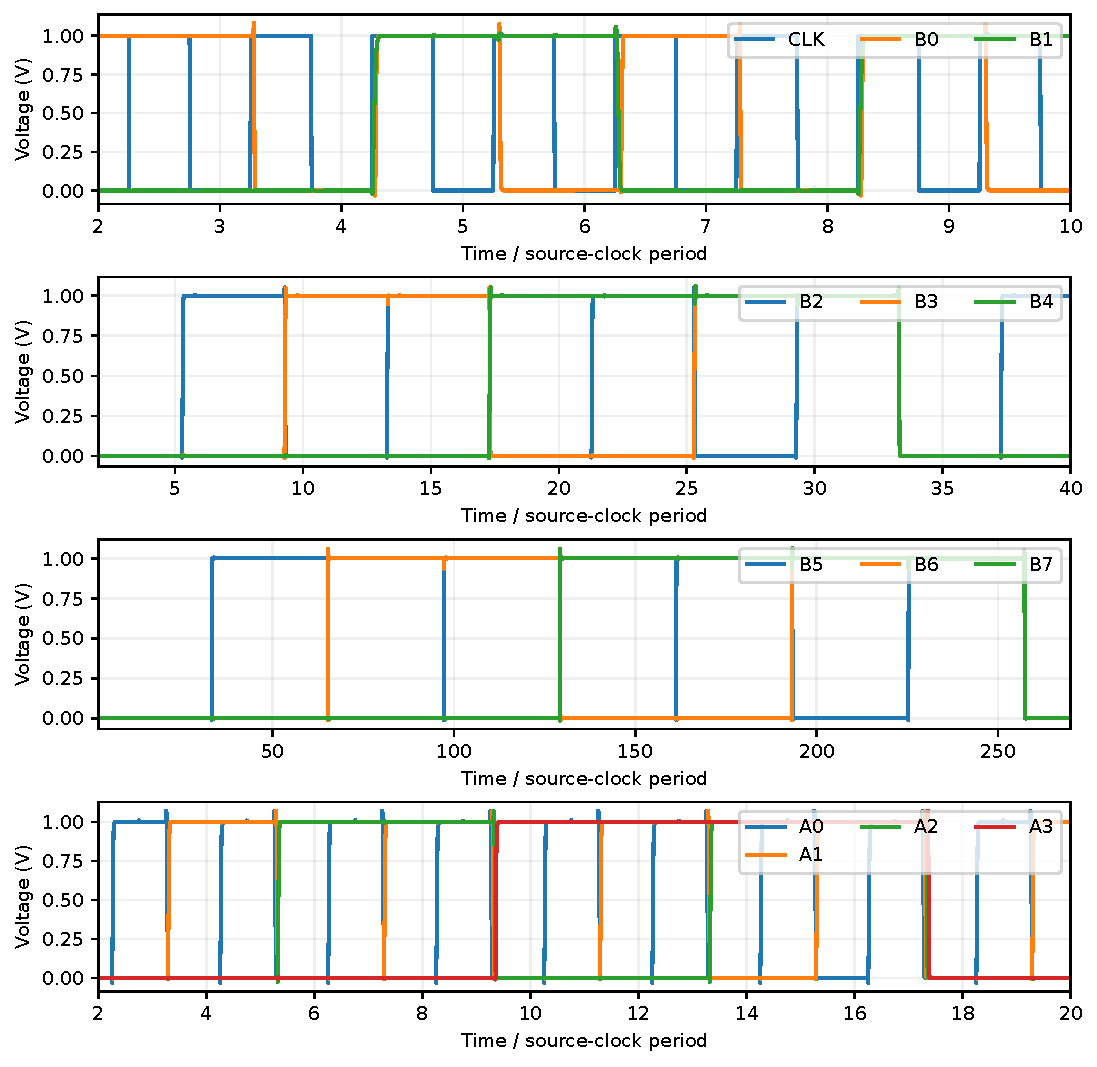
\includegraphics[width=.94\linewidth]{figures/division_waveforms.pdf}
\caption{Baseline divider waveforms; time windows differ between panels.}
\end{figure}

In the ripple 7-to-8 transition, A0, A1, A2 and A3 cross half supply approximately 0.532, 1.182, 1.816 and 2.263 ns after the source edge, respectively. The selected synchronous B2/B3/B4 transition occurs around 1.012 ns without the same bit-by-bit delay accumulation. These values are interpolated from T/200 printed data and are limited by the 100 ps baseline sample interval; picosecond signoff precision is not claimed.

\begin{figure}[htbp]\centering
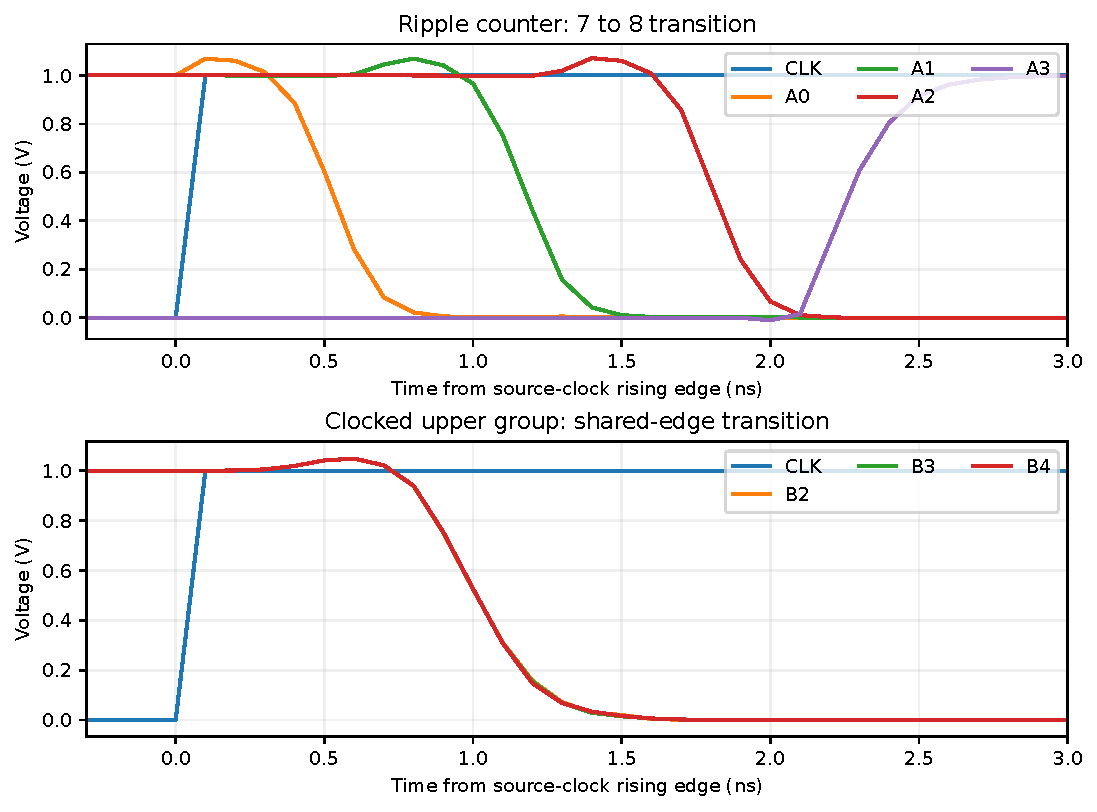
\includegraphics[width=.94\linewidth]{figures/transition_alignment.pdf}
\caption{Accumulated ripple delay and the shared transition of a synchronous group.}
\end{figure}

\section{Frequency boundary and power}

\begin{center}\small
\begin{tabular}{lrrr}
\toprule
T (ns) & f (MHz) & Sync correct/260 & Ripple correct/260 \\
\midrule
20 & 50.0 & 260 & 260 \\
10 & 100.0 & 260 & 260 \\
6 & 166.7 & 260 & 260 \\
5 & 200.0 & 260 & 228 \\
3 & 333.3 & 260 & 195 \\
2.5 & 400.0 & 130 & 130 \\
2 & 500.0 & 130 & 130 \\
1.5 & 666.7 & 0 & 97 \\
1 & 1000.0 & 0 & 0 \\
\bottomrule
\end{tabular}
\end{center}

The highest tested frequencies with 260/260 correct words are 333.3/166.7 MHz for synchronous/ripple. The next tested failing points are 400.0/200.0 MHz. These are finite-sweep boundaries at the stated load, 20 ps edges, and 0.45T settling deadline, not unconditional maximum frequencies across PVT.

\begin{figure}[htbp]\centering
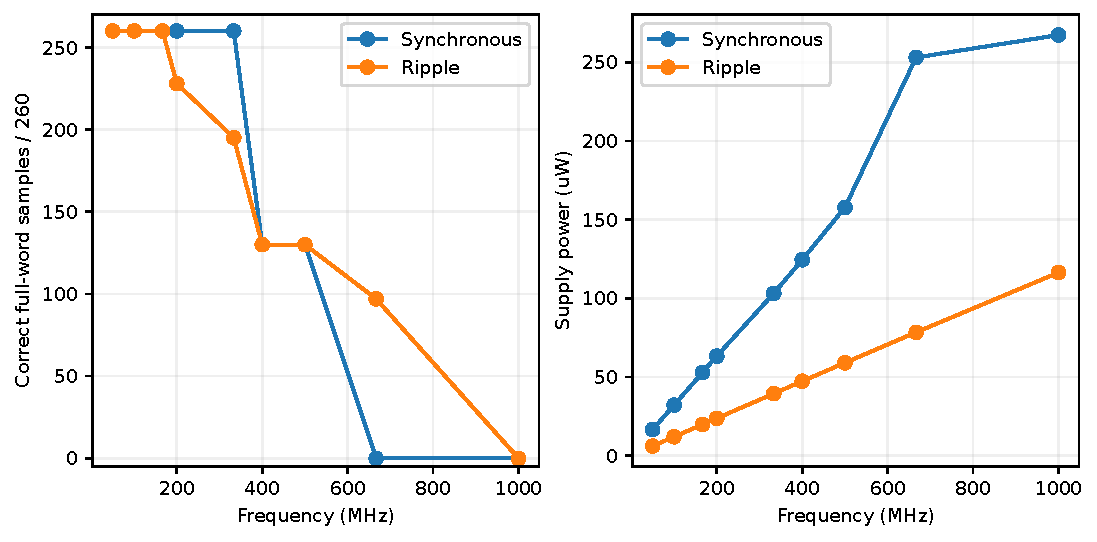
\includegraphics[width=.94\linewidth]{figures/frequency_and_power.pdf}
\caption{Sample correctness and supply power; power at failing frequencies is retained and is not valid-operation efficiency.}
\end{figure}

\begin{center}\small
\begin{tabular}{lrrr}
\toprule
Architecture & Transistors & Clock edge charge (fC) & 50 MHz power (µW) \\
\midrule
Sync (8 outputs) & 414 & 60.450 & 16.508 \\
Ripple (4 bits) & 98 & 13.474 & 6.034 \\
\bottomrule
\end{tabular}
\end{center}

Transistor counts recursively expand the instantiated hierarchy, including clock inverters, synchronizers, reset, and XOR/AND logic, while excluding unused subcircuits. Clock loading integrates independent 0 V probe currents during the rising edge at 10.25T. At a 1 V swing, Q/ΔV corresponds to approximately 60.450/13.474 fF of edge-specific effective loading, not layout capacitance. Power averages supply input from 10T to 270T and excludes ideal clock/reset source power.

\section{Discussion and limitations}

The synchronous architecture trades additional clock loading and logic for reduced sequential propagation, while ripple reduces direct clock loading but waits for preceding transitions. The handout compares different sizes, eight outputs versus four bits, so total power is not an equal-function/equal-width efficiency comparison. Results are not forced to reproduce the original 1 GHz/500 MHz process examples, and ideal counters are not used to conceal frequency failures. Per-case waveforms, full-word validation, and measurements are retained in results.
